%\documentclass[%
%% border=1pt
%  border={0pt 0pt 0pt 0pt} % left bottom right top
%]{standalone}
%\usepackage{tikz} % Required for drawing custom shapes
%\usepackage{pgfplots}
%\pgfplotsset{compat = newest}
%
%\usepackage{amsbsy}
%\usetikzlibrary{decorations.pathreplacing,calc}
%\usetikzlibrary{shapes}
%\usepackage{amsmath,stackrel}
%\usetikzlibrary{arrows.meta}
%\usetikzlibrary{arrows}
%\usetikzlibrary{calc}
%\usetikzlibrary{math}
%
%\begin{document}
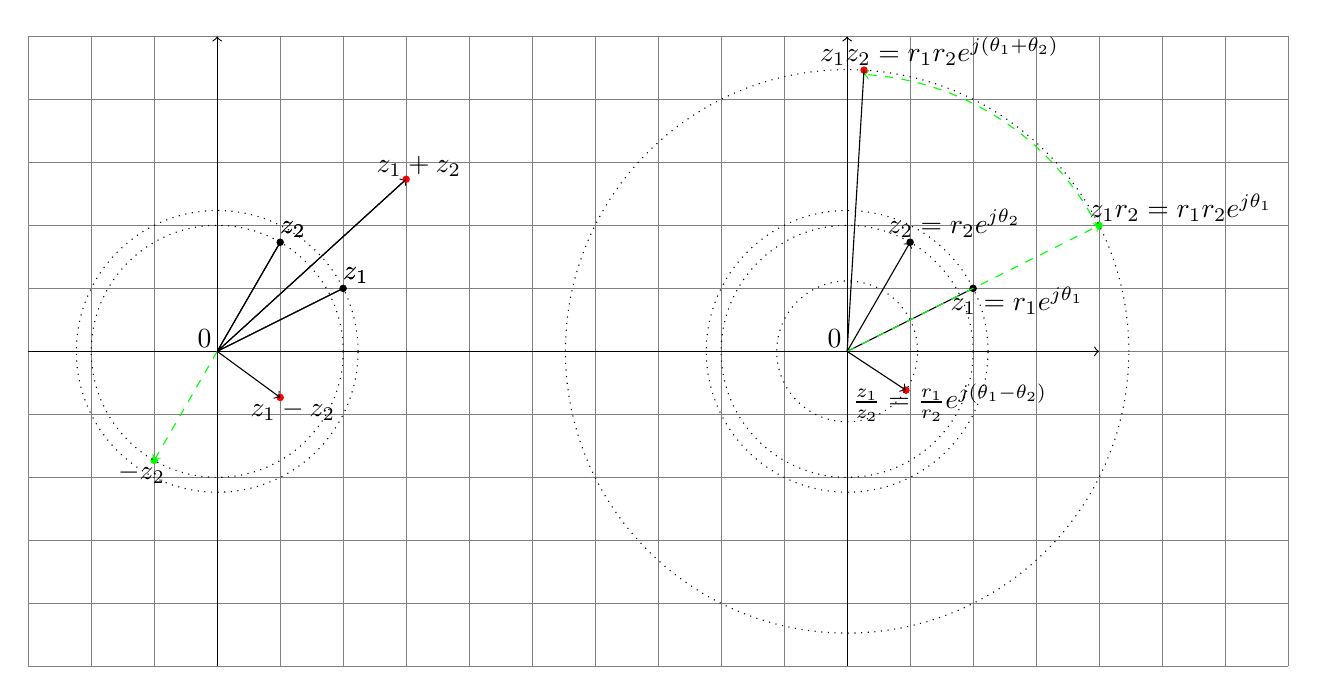
\begin{tikzpicture}[scale=0.8]
\draw[style=help lines] (-5,-5) grid (15,5);
\draw[black,->] (-5,0) -- (12,0);
\draw[black,->] (0-2,-5) -- (0-2,5);

\draw[fill] (2-2,1) circle[radius=0.05];
\draw[fill] (1-2,1.732) circle[radius=0.05];
\draw[fill,green] (-1-2,-1.732) circle[radius=0.05];
\node at (1.2-2,1.932) {$z_2$};
\node at (2.2-2,1.2) {$z_1$};
\node at (-1.2-2,-1.932) {$-z_2$};

\draw[->] (0-2,0) -- (2-2,1) (0-2,0) -- (1-2,1.732) (0-2,0) -- (3-2,2.732);
\draw[->,green,dashed] (0-2,0) -- (-1-2,-1.732);

\draw[fill,red] (3-2,2.732) circle[radius=0.05];
\draw[fill,red] (1-2,-0.732) circle[radius=0.05];

%\draw[fill,red] ({0.46*360/(2*pi)+60}:{2*sqrt(5)}) circle[radius=0.05];
%\draw[fill,red] ({0.46*360/(2*pi)-60}:{sqrt(5)/2}) circle[radius=0.05];

\draw[dotted] (0-2,0) circle[radius={sqrt(5)}];
\draw[dotted] (0-2,0) circle[radius=2];

\node at (1.2-2,1.932) {$z_2$};
\node at (2.2-2,1.2) {$z_1$};
\node at (3.2-2,2.932){$z_1+z_2$};
\node at (1.2-2,-0.932){$z_1-z_2$};
\draw[->] (0-2,0) -- (2-2,1) (0-2,0) -- (1-2,1.732) (0-2,0) -- (3-2,2.732) (0-2,0) -- (1-2,-0.732);
\node at (-0.2-2,0.2) {0};
%---------------------------------------------------------------------------------------------------
%\draw[black,->] (1,0) -- (10,0);
\draw[black,->] (8,-5) -- (8,5);

\draw[fill] (10,1) circle[radius=0.05];
\draw[fill] (9,1.732) circle[radius=0.05];
\draw[fill,green] (12,2) circle[radius=0.05];

\node at (9.2+0.5,1.932+0.1) {$z_2 = r_2 e^{j \theta_2}$};
\node at (10.2+0.5,1.2-0.4) {$z_1 = r_1 e^{j \theta_1}$};
\node at (12.2+1.1,1.932+0.35) {$z_1 r_2 = r_1 r_2 e^{j \theta_1}$};

\draw[->] (8,0) -- (10,1) (8,0) -- (9,1.732);
\draw[dashed,green,->] (8,0) -- (12,2);
%\draw[->] (26.5:{2*sqrt(5)}) arc (86.5:{2*sqrt(5)});
\draw[dashed,green,->] (12,1.932) arc[start angle=26.56505, end angle=60+26.56505,radius=4.472cm];

\draw[fill,red] (8.2679,4.4641) circle[radius=0.05];
\draw[fill,red] (8.9330,-0.6160) circle[radius=0.05];

%\draw[fill,red] ({0.46*360/(2*pi)+60}:{2*sqrt(5)}) circle[radius=0.05];
%\draw[fill,red] ({0.46*360/(2*pi)-60}:{sqrt(5)/2}) circle[radius=0.05];
\draw[dotted] (8,0) circle[radius=2];
\draw[dotted] (8,0) circle[radius={sqrt(5)}];
\draw[dotted] (8,0) circle[radius={2*sqrt(5)}];
\draw[dotted] (8,0) circle[radius={sqrt(5)/2}];

\node at (8.2679+1+0.2,4.4641+0.3){$z_1 z_2 = r_1 r_2 e^{j (\theta_1+\theta_2)}$};
\node at (8.9330+.2+0.5,-0.6160-0.2){$\frac{z_1}{z_2} = \frac{r_1}{r_2} e^{j (\theta_1 - \theta_2)}$};
\draw[->] (8,0) -- (8.2679,4.4641) (8,0) -- (8.9330,-0.6160);
\node at (8-0.2,0.2) {0};
\end{tikzpicture}
%\end{document} 